%!TEX root = Thesis.tex

\chapter{Coordination Complexes with Silver}
\chaptermark{Silver}
\label{ch:silver}

Silver has been used for centuries due to its significant antimicrobial properties.  Silver and silver nanoparticles are used in a wide range of health and food applications.  \fixme{find the article from wikipedia to cite here}  Silver coordination complexes have also show biological activity.  \emph{Bis}-diphosphine silver complexes have shown anti-tumour and anti-fungal activity.\cite{Berners-Price1988, Liu2008}

Silver is used industrially as a catalyst to convert ethene to ethylene glycol on an industrial scale.  It is also often used in the control rods of nuclear reactors.  Silver has also found use as a component in the Oddy test.  This test is used to determine if materials give off gases which may be harmful to art and historical artefacts, specifically the silver is used to detect reduced sulfur and sulfur carbonyl compounds.  \fixme{this needs some citations}

Furthermore  silver complexes have gained attention recently as potential catalysts in a number of transformations including Si-H activation\cite{Iglesias2012} asymmetric aldol conversions \cite{Sawamura1990} and allylation of benzaldehyde\cite{Malaise2006, Yanagisawa1999}.

The coordination chemistry of silver is interesting due a high degree of geometrical flexibility. The bite angle, electronic influence of the diphosphine, and the coordination mode of ancillary ligands can all impact the type of complex formed and even with the relatively straightforward equimolar stoichiometry an array of different structures have been reported.  For a good overview see Meijboom et al.\cite{Meijboom2009}.  Silver is also useful to study as it consists of two spin \nicefrac{1}{2} isotopes \Agseven{} and \Agnine{} with abundances of 51.85\% and 48.18\% respectively.  Hence additional information can be gained from the value of the \JAgP{}.

\begin{figure}[h]
\begin{center}
\vspace{0.5cm}
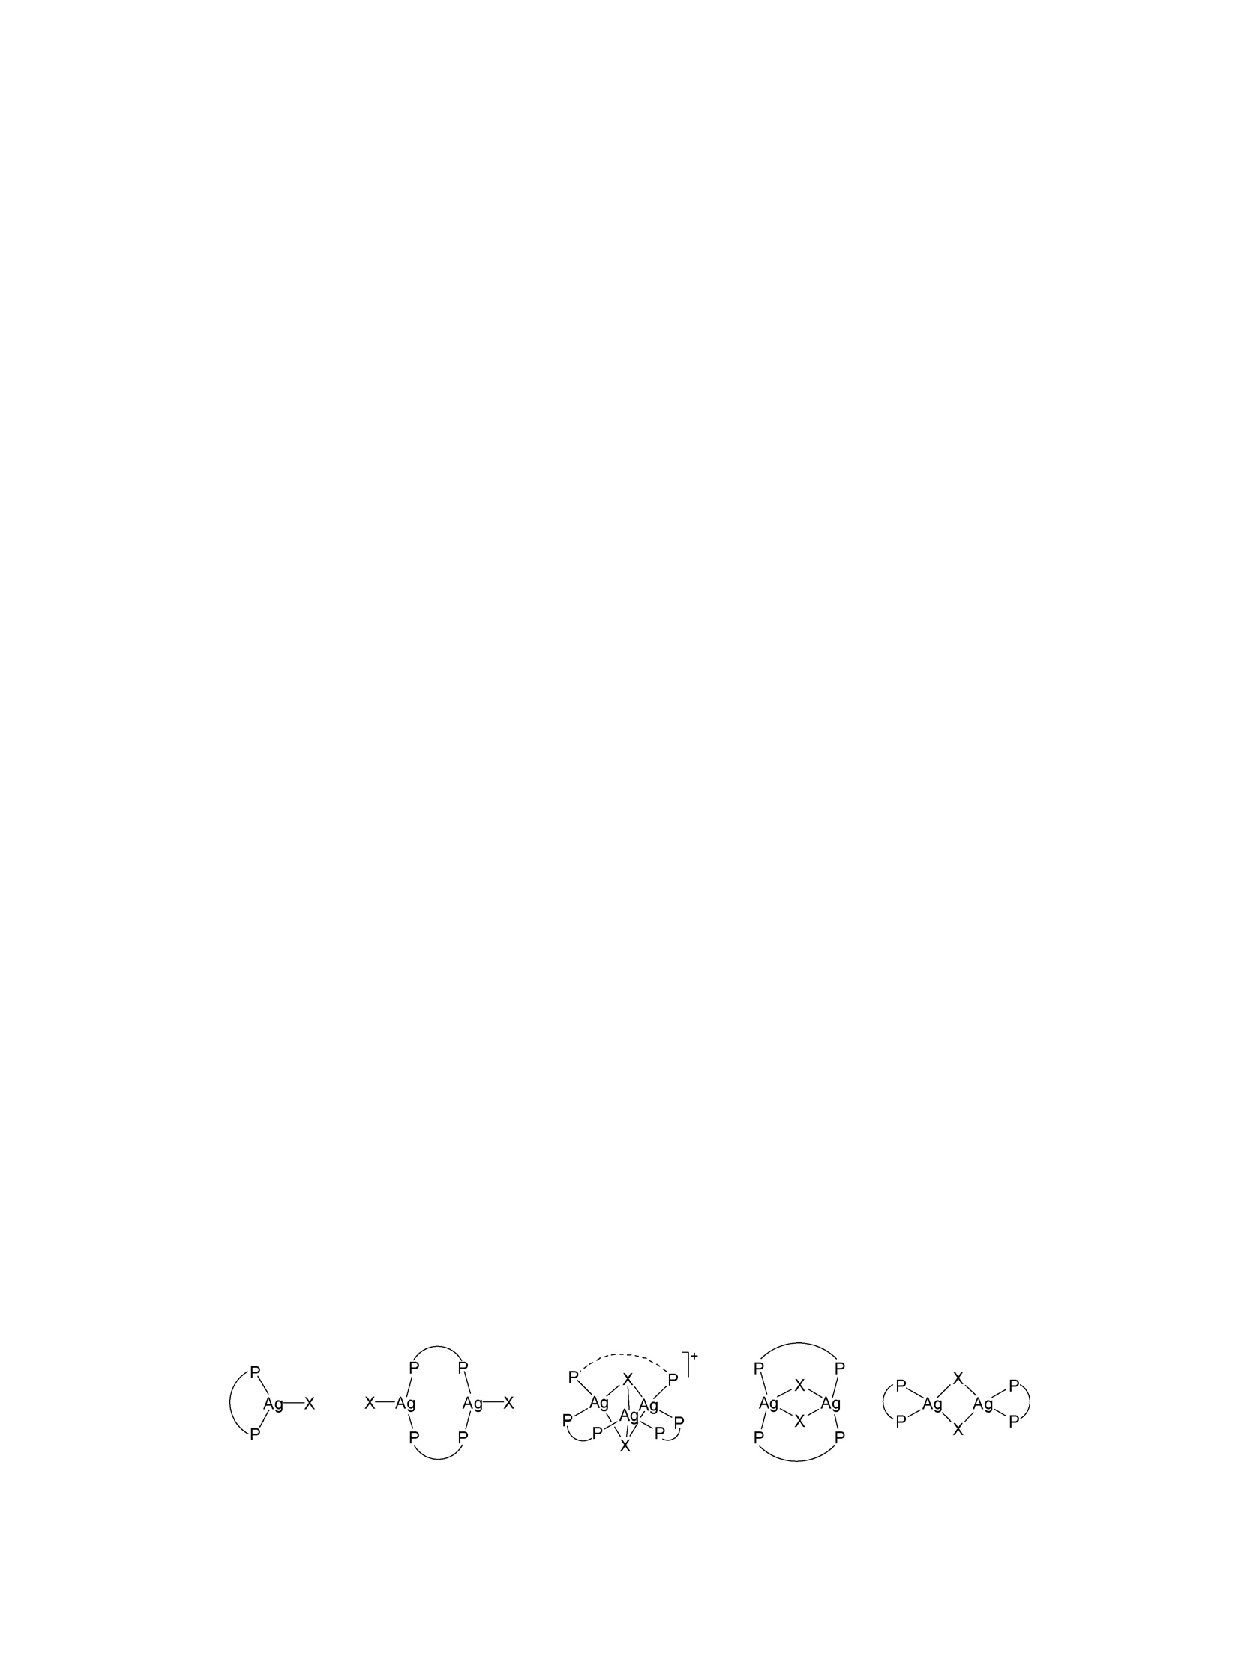
\includegraphics{../Figures/Possiblesilverstructures.pdf}
\caption[Possible general structures for 1:1 silver diphosphine complexes]{Possible general structures for 1:1 silver diphosphine complexes, reproduced from Meijboom et al.\cite{Meijboom2009}}
\vspace{0.2cm}
\label{Silverstructures}
\end{center}
\end{figure}
\vspace{0.2cm}

%In addition to forming unusual coordination environments silver complexes have also been extensively studied due to their biological activity.  Bisdiphosphine silver complexes have shown anti-tumour and anti-fungal activity.\cite{Berners-Price1988, Liu2008} A recent study (Liu2008) showed that silver complexes of bidentate pyridyl phosphines showed in vitro anti-tumour activity.  

Silver complexes of xanthene backboned ligands have been reported previously.\cite{Malaise2006, Balakrishna2008}  The reported complexes are all trigonal geometries with the general formula [AgLX] where X = a negatively charged ligand OTf-, BF4 for Malaise2006,  and L = the bidentate xanthene ligand.  Of most relevance to this work is the complex [AgBr(xantphos)] reported by Kaltzoglou.\cite{Kaltzoglou2007}  This complex exists as a monomeric species with a P-Ag-P angle of 109.38\degrees{}, very close to the natural bite-angle for xantphos (111.7\degrees).\cite{Kranenburg1995}  The complex reacted with a heterocyclic thione forming the tetrahedral species [AgBr(xantphos)(py2SH)].  The P-Ag-P angle for this is increased slightly to 111.51\degrees{}.  The steric bulk of the xantphos ligand was proposed as the reason for the lack of chelation.

\fixme{Why don't the commas and full-stops look nice under the degrees symbol?}

Similar complexes to \fixme{insert reference to the xantphos one} were synthesised for the sulfur, silicon and carbon bridged tBu-xantphos ligands.  The ligands were reacted with silver chloride in the dark and generated the expected [AgCl(L)] complexes.  The \phosphorus{} NMR spectra showed the expected pair of doublets in all cases as summarised in Table~\ref{table:silverchlorides}.  All had mass spectra that showed a clear peak for [M-Cl-]+ with no sign of any dimeric species, clearly indicating a monomeric species.  

\begin{scheme}[h]
\begin{center}
\vspace{0.5cm}
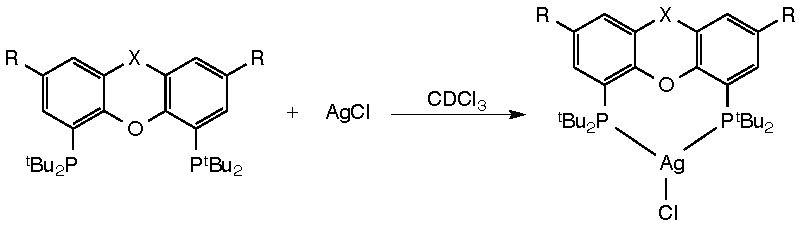
\includegraphics{../Schemes/Silverchloridescheme.pdf}
\caption[Reaction of silver chloride with \tBuxantphos\ ligands]{Reaction of silver chloride with \tBuxantphos\ ligands}
\vspace{0.2cm}
\label{Silverchloride}
\end{center}
\end{scheme}
\vspace{0.2cm}

\begin{table}[h]
\caption[Selected NMR data of silver diphosphine complexes]{Selected NMR data of silver diphosphine complexes} 
\vspace{1em}
\label{table:silverchlorides}
\small
\begin{center}
\begin{tabular}{ c c c c c}
	\toprule{}
	~~Compound~~&~~$\delta$\phosphorus{}$/$ppm~~&~~$\Delta\delta$~~&~~\JAgPseven{}$/$Hz~~&~~\JAgPnine{}$/$Hz~~\\
	\midrule{}
	~~SitBu~~&~~24.2~~&~~15.8~~&~~408.1~~&~~471.1~~\\
	~~StBu~~&~~21.8~~&~~12.3~~&~~406.7~~&~~469.6~~\\
	~~CtBu~~&~~20.7~~&~~10.5~~&~~409.3~~&~~472.2~~\\
	\bottomrule{}
\end{tabular}
\end{center}
\end{table}

\fixme{check this paragraph with the actual crystal structure}\\
Silver thixantphos chloride was successfully crystallised as colourless crystals in the \fixme{P21} space group (Figure \ref{crystalthixantphossilverchloride}).  Selected bond lengths and angles, and crystallographic data are given in Tables \ref{table:crystalthixantphossilverchloride:lengths} and \ref{table:crystalthixantphossilverchloride:data} respectively.  The X-ray crystal structure shows a trigonal planar structure with the P-Ag-P angle of 130.4\degrees moderately distorted from the ideal trigonal planar structure.  The Ag-O distance is well outside the sum of the van der waals radii indicating no interaction between the two atoms.  The bite-angle is very close to the natural bite-angle calculated for tBu-thixantphos as 131.4\degrees.  As such the coordination geometry is likely driven very much by ligand effects rather than the silver or the chloride.  Silver can form a huge array of different coordination geometries and generally the preferred structure is controlled by ligand effects.\fixme{get a citation}

\begin{figure}[hp]
\begin{center}
\vspace{0.5cm}
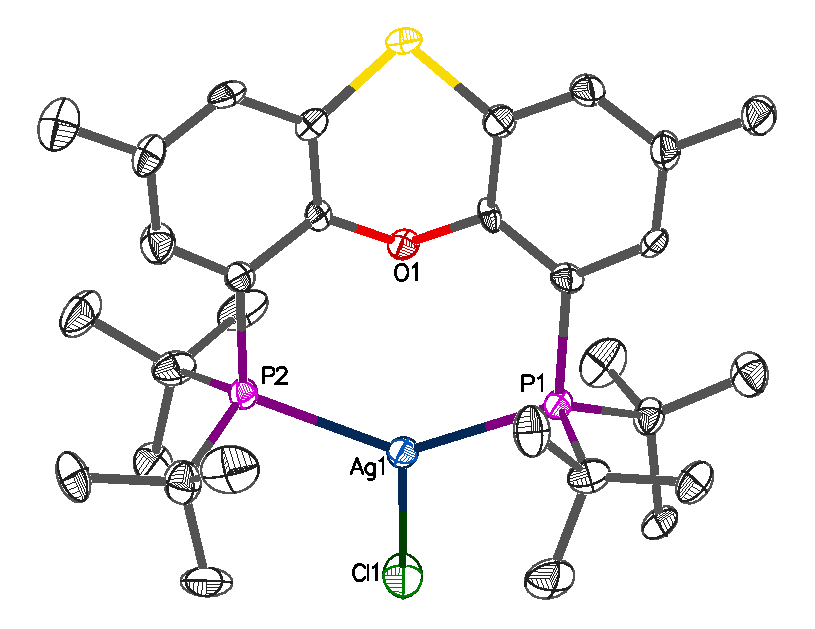
\includegraphics[scale=0.8]{../Figures/Crystalthixantphossilverchloride.pdf}
\caption[X-ray crystal structure of \ce{[Ag(tBu-thixantphos)Cl]}]{X-ray crystal structure of \ce{[Ag(tBu-thixantphos)Cl]}, hydrogen atoms omitted for clarity}
\vspace{0.2cm}
\label{crystalthixantphossilverchloride}
\vspace{0.2cm}
\end{center}
\end{figure}
\vspace{0.2cm}

\begin{figure}[hp]
\begin{center}
\vspace{0.5cm}
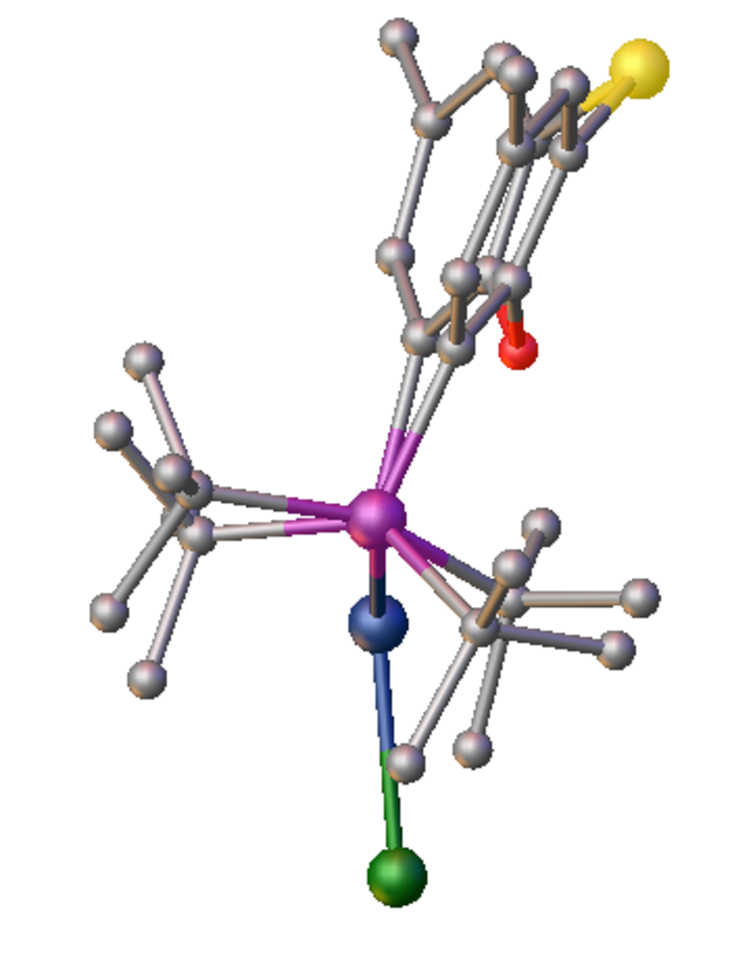
\includegraphics[scale=0.8]{../Figures/Crystalthixantphossilverchloridesideview.pdf}
\caption[X-ray crystal structure of \ce{[Ag(tBu-thixantphos)Cl]}, side view]{X-ray crystal structure of \ce{[Ag(tBu-thixantphos)Cl]}, side view}
\vspace{0.2cm}
\label{crystalthixantphossilverchloride:sideview}
\end{center}
\end{figure}
\vspace{0.2cm}

\begin{table}[ht]
\caption[Selected bond distances (\AA) and angles (\degrees) of \ce{[Ag(tBu-thixantphos)Cl]}]{Selected bond distances (\AA) and angles (\degrees) of \ce{[Ag(tBu-thixantphos)Cl]}} 
\vspace{1em}
\label{table:crystalthixantphossilverchloride:lengths}
\small
\begin{center}
\begin{tabular}{l l l l}
	\toprule
	\multicolumn{2}{l}{\bfseries{~Bond distances (\si{\angstrom})}} & \multicolumn{2}{c}{\bfseries{Bond angles (\degrees)}} \\
	\midrule		
	~P1-P2		~~&~~4.416(3)~~	&~~P1-Pt-P2			&~~130.50(7)~~	\\	
	~P1-Ag		~~&~~2.430(2)~~	&~~P1-Ag-Cl			&~~116.46(8)~~	\\
	~P2-Ag		~~&~~2.433(2)~~	&~~P2-Ag-Cl			&~~112.95(8)~~	\\
	~Ag-O		~~&~~3.007(6)~~	&~~Ring 1-Ring 2		&~~35.7(3)~~		\\
	~Ag-Cl		~~&~~2.491(2)~~	&~~					&~~		~~		\\
	\bottomrule{}
\end{tabular}
\end{center}
\end{table}

\begin{table}[htp]
\small
\caption[Crystallographic Data and Structure Refinement of \ce{[Ag(\tButhixantphos)Cl]}]{Crystallographic Data and Structure Refinement of \ce{[Ag(\tButhixantphos)Cl]}} 
\vspace{1em}
\label{table:crystalthixantphossilverchloride:data}
\small
\begin{center}
\begin{tabular}{l l}
	\toprule
	\bfseries{Empirical formula}~~& \bfseries{\ce{C30H46AgClOP2S}}\\
	\midrule
	Formula weight	 							& 659.99\\
	Temperature/K	 							& 285.47(10)\\
	Crystal system	 							& monoclinic\\
	Space group	 							& P2\sub{1}\\
	a$/$\si{\angstrom}							& 8.6697(3)\\
	b$/$\si{\angstrom} 							& 15.4417(6))\\
	c$/$\si{\angstrom}							& 11.9482(4)\\
	$\alpha/$\degrees							& 90\\
	$\beta/$\degrees							& 99.700(3)\\
	$\gamma/$\degrees							& 90\\
	Volume$/$\si{\angstrom\cubed}  				& 1576.70(10)\\
	Z	 									& 2\\
$\rho$\sub{calc} \si{\milli\gram}$/$\si{\milli\metre\cubed} 	& 1.390\\
\si{\metre}$/$\si{\milli\metre} 						& 7.636\\
F(000)	 									& 688.0\\
Crystal size$/$\si{\milli\metre\cubed}	 				& 0.3842 x 0.3421 x 0.1062\\
Radiation	 									& CuK$\alpha$ ($\lambda$ = 1.54184)\\
2$\theta$ range for data collection					& 7.506 to 147.890\degrees\\
Index ranges	 								& -10 $\leq$ h $\leq$ 10, -19 $\leq$ k $\leq$ 16, -14 $\leq$ l $\leq$ 14\\
Reflections collected	 							& 12454\\
Independent reflections	 						& 5818 [R\sub{int} = 0.0724, R\sub{sigma} = 0.0651]\\
Data$/$restraints$/$parameters					& 5818$/$1$/$339\\
Goodness-of-fit on F$^{2}$	 					& 1.138\\
Final R indexes [I$>$=2$\sigma$ (I)]	 				& R\sub{1} = 0.0545, wR\sub{2} = 0.1579\\
Final R indexes [all data]	 						& R\sub{1} = 0.0563, wR\sub{2} = 0.1618\\
Largest diff. peak/hole / e \si{\per\angstrom\cubed}		& 0.88/-1.78	\\
Flack parameter								& -0.016(13)	\\
	\bottomrule
\end{tabular}
\end{center}
\end{table}

In the solid state structure of silver tBu-thixantphos chloride the backbone shows a significant degree of twisting \fixme{get some info about how much twisting is present} and is bent to give two distinct halves of the molecule.  The chloride is on the convex side of the molecule rather than the \fixme{less sterically hindered - check this} concave side and is not perfectly centred with a difference in the P-Ag-Cl angles of 3.49\degrees{}.  This difference is likely due to the backbone twisting and the chloride occupying the least sterically hindered space.  This structure would result in two distinct sets of t-Bu groups, the two on the convex face and the two on the concave face.  However, this is not observed in the NMR spectra.\fixme{the NMR of the tBu is a bit of a mess and I need to look at it again}  This indicates that the backbone is not static in solution but is inverting on the NMR timescale such that the signals for the two t-Bu environments average and only a single t-Bu \proton{} resonance and two t-Bu \carbon{} resonances are observed.  

Given the clear similarities of the three complexes (see Table~\ref{table:silverchlorides}) it is likely that the SitBu and CtBu complexes also display trigonal complexes with no oxygen interaction.  The changes in \JAgP{} appear unrelated to the natural bite angle calculated for the three ligands \fixme{refer to that section?}.  

Complexes of the type \ce{[Ag(L)]BF4} were synthesised in the hope that the oxygen would successfully displace the weakly bound \ce{BF4-}.  Due to the halophilic natural of silver the typically considered non-coordinating \ce{BF4-} counterions can bond to the metal centre through one of the fluorine atoms.  Previous reports have shown that even in the presence of potentially coordinating oxygen atoms a linear diphosphine complex was formed instead without \ce{BF4-} or the ether backbone coordinating.\cite{Heuer2000, Camalli1984}  With the tBu-xantphos ligands a single resonance in the \fluorine{} NMR spectrum (with two signals due to the \Bten{} and \Beleven{} isotopomers) was observed in the position expected for a non-coordinating \ce{BF4-}.  However no evidence for oxygen coordination was found.  As such it is likely that similar to previous reports the structure is an electron-deficient 14-electron silver diphosphine linear complex.  

\begin{scheme}[h]
\begin{center}
\vspace{0.5cm}
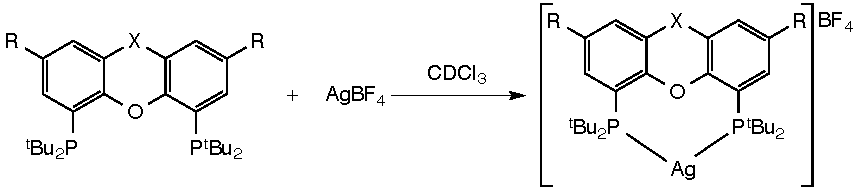
\includegraphics{../Schemes/SilverBF4scheme.pdf}
\caption[Reaction of silver tetrafluoroborate with \tBuxantphos\ ligands]{Reaction of silver tetrafluoroborate with \tBuxantphos\ ligands}
\vspace{0.2cm}
\label{SilverBF4}
\end{center}
\end{scheme}
\vspace{0.2cm}


\begin{table}[h]
\caption[Selected NMR data of silver tetrafluoroborate complexes]{Selected NMR data of silver tetrafluoroborate complexes} 
\vspace{1em}
\label{table:silverBF4}
\small
\begin{center}
\begin{tabular}{ c c c c c}
	\toprule{}
	~~Compound~~&~~$\delta$\phosphorus{}$/$ppm~~&~~$\Delta\delta$ ppm~~&~~\JAgPseven{}$/$Hz~~&~~\JAgPnine{}$/$Hz~~\\
	\midrule{}
	~~SitBu~~&~~31.5~~&~~23.1~~&~~482.9~~&~~557.4~~\\
	~~StBu~~&~~28.4~~&~~18.9~~&~~486.7~~&~~562.2~~\\
	~~CtBu~~&~~27.6~~&~~17.4~~&~~486.3~~&~~561.1~~\\
	\bottomrule{}
\end{tabular}
\end{center}
\end{table}

14-electron silver complexes are relatively unusual due to the ability of silver to form a large number of different coordination geometries including a large number of possible dimers.  We do not see any evidence of a dimer, trimer or higher order oligiomer in the mass spectrum \fixme{would this have the same m/z though?} or in the \phosphorus{} NMR spectrum as we may expect to see additional silver coupling.  As such a monomeric 14-electron diphosphine complex is proposed as the product of the reaction between \ce{AgBF4} and the tBu-xantphos ligands.  

\fixme{consider changing the StBu etc. to complex references}

See Derrah2012, Freudenmann2011, Hollander1976 - bis DPEphos Ag
Kaltzoglou2007, 
Camalli1984

Methanol at -20'C for 4 hours then at RT for 20 h
low ee (18\% and conversion of 68\%) 
no ee with PN ligands

According to Pregosin (find a reference?) the values for d10 complexes the coupling constants decrease with increasing coordination so a species that is two-coordinate will have a larger coupling constant than one that is four-coordinate.

Socol1984
Meijboom

